% define document type (i.e., template. Here: A4 APA manuscript with 12pt font)
\documentclass[man, 12pt, a4paper]{apa7}

% add packages
\usepackage[american]{babel}
\usepackage[utf8]{inputenc}
\usepackage{csquotes}
\usepackage{hyperref}
\usepackage[style=apa, sortcites=true, sorting=nyt, backend=biber, natbib=true, uniquename=false, uniquelist=false, useprefix=true]{biblatex}
\usepackage{authblk}
\usepackage{graphicx}
\usepackage{setspace,caption}
\usepackage{subcaption}
\usepackage{enumitem}
\usepackage{lipsum}
\usepackage{soul}
\usepackage{xcolor}
\usepackage{fourier}
\usepackage{stackengine}
\usepackage{scalerel}
\usepackage{fontawesome}
\usepackage[normalem]{ulem}
\usepackage{longtable}
\usepackage{amsmath}
\usepackage{afterpage}
\usepackage{float}
\usepackage{titling}
\usepackage{censor}
\usepackage{tcolorbox}
\usepackage{pdfpages}

% formatting links in the PDF file
\hypersetup{
pdfpagemode={UseOutlines},
bookmarksopen=true,
bookmarksopenlevel=0,
hypertexnames=false,
colorlinks   = true, %Colours links instead of ugly boxes
urlcolor     = blue, %Colour for external hyperlinks
linkcolor    = blue, %Colour of internal links
citecolor   = cyan, %Colour of citations
pdfstartview={FitV},
unicode,
breaklinks=true,
}

% language settings
\DeclareLanguageMapping{american}{american-apa}

% add reference library file
\addbibresource{references.bib}

% Title and header
\title{Supplemental Information X: Acculturation Focus Group Discussion Methodology}
\shorttitle{SI X: Acculturation Focus Group Discussion}
%\author{Jannis Kreienkamp, Laura F. Bringmann, Raili F. Engler, Peter de Jonge, Kai Epstude}
\author{[authors masked for peer review]}

% set indentation size
\setlength\parindent{1.27cm}

% adapt table and figure labels
\setcounter{equation}{0}
\setcounter{figure}{0}
\setcounter{table}{0}
\setcounter{page}{1}
\makeatletter
\renewcommand{\theequation}{S\arabic{equation}}
\renewcommand{\thefigure}{S\arabic{figure}}
\renewcommand{\thetable}{S\arabic{table}}

% Start of the main document:
\begin{document}

% add title information (incl. title page and abstract)
\begin{titlepage}
	{\noindent\Large Supplementary Information for \par}
	\vspace{0.5cm}
	{\noindent\Large The Migration Experience: A Conceptual Framework and Systematic Review of Psychological Acculturation\par}
	\vspace{1.5cm}
	{\noindent\LARGE\bfseries \thetitle \par}
	\vspace{2cm}
	{\noindent\Large\itshape \theauthor \par}
	\vfill
	%\noindent Corresponding Author: Jannis Kreienkamp\par
	%\noindent E-mail: j.kreienkamp@rug.nl\par
	\noindent Corresponding Author: [masked for peer review]\par
	\noindent E-mail: [masked for peer review]\par
	\vfill

    % Bottom of the page
	{\noindent Last updated: \today\par}
\end{titlepage}

% add title again on page 1 (after title page)
\begin{center}
   \textbf{\thetitle} 
\end{center}

This supplemental material aims to provide additional methodological details of the preliminary focus group discussion reported in the main text. The focus group discussion itself was the first study in a larger collaboration between our university research team and a local refugee resettlement agency. The main aim of the focus group discussion was to gain an in-depth, bottom-up, and practical understanding of how psychological acculturation is conceptualized and addressed by key players in Dutch society. To this aim we invited a broad and diverse set of societal actors involved in the acculturation process. Below we introduce the methodological and analytical approaches in more detail.

\section{Methods}

Given that focus group discussions are not a standardized procedure \citep[][]{Morgan2010, Barbour2001}, we will sequentially describe the study design, the participants, the study setting, and the data collection. 

\subsection{Study Design}

We conducted the focus group discussion as a single cross-sectional round table event. We then followed the study up with a literature study and systematic scoping review (see main text). We chose this particular design to address our main aims and research questions. In particular, the focus group allowed us to bring together a diverse set of key societal actors involved in the acculturation process and explore the discourse of how acculturation is conceptualized in practice.

\subsection{Participants}

The focus group discussion was hosted jointly by a university in the Netherlands and the local refugee resettlement organization as part of a larger ongoing collaboration. The participants were purposefully selected and invited to represent the broad diversity of people involved in the acculturation process. Our purposeful sampling criteria focused on diversity in terms of gender, age, field and service provided, migration type, professional status, and job seniority. The participants were contacted by the main coordinator at the refugee resettlement organization (a copy of the invitation letter is attached in \hyperref[app:AppendixInvitation]{Appendix \ref*{app:AppendixInvitation}}). None of the forced migrants invited were still clients of the resettlement organization. The focus group discussion ultimately consisted of 12 people (including three trained moderators). 

Given the small sample size of a focus group discussion and to uphold participant confidentiality and data privacy, we will describe participant demographic information in broader categories only. Of the twelve participating people, six were women and six were men (including moderators). The nine participants consisted of five women and four men. The age of the participants ranged from 26 to 68. The group included three migrants and nine members of the local majority group.

\subsubsection{Facilitators and Moderators}

Three researchers were present during the focus group discussion with differing degrees of participation in the focus group discussion. A senior member of the research team acted as the main facilitator of the event, guiding and chairing the discussion. A second researcher acted as the moderator, introducing the the topic as well as structured and follow-up questions. The third researcher was mainly a participatory observant, but also took notes and asked clarification and follow-up questions.

\subsubsection{Acculturation Partners}

The societal partners who were involved in migrant acculturation were diverse in their age, education, and profession. We invited both professional and volunteer workers and aimed to include most relevant service providers for recent migrants. As a result, our societal partners worked in the fields of (language) education, naturalization, administration, politics, as well as cultural orientation. Our participants had a diverse set of responsibilities and worked as teachers and educators, coaches and counselors, administrators and coordinators, as well as volunteers and researchers. Notably some of our participants fulfilled multiple roles in their work (e.g., language teacher and naturalization course coordinator, or administrator and volunteer).

\subsubsection{Migrants}

The three migrants were predominantly male and younger than the majority of the acculturation partners. The migrant group included two forced migrants and one voluntary migrant. The individual duration of residency was between four and five years and the forced migrants were granted legal asylum status approximately three and a half years prior to the focus group study. None of the three migrants were fully naturalized at the time of the study. The countries of origin were Germany, Syria, and Sudan. We chose the three countries for their relative difficulty of adjusting to the Netherlands (in terms of cultural distance as well as differences in literacy, education level, and reception). Two of the three migrants had some form of university education and two of the three migrants arrived alone while the third arrived with their family. 

\subsection{Study Setting}

The study itself was conducted in a conference room of the university. We chose the location as a neutral room for all parties, as an easily accessible building, and to retain control over the audio recording quality. We invited participants to join the focus group discussion in the early evening to accommodate the schedules of working participants and offered culturally appropriate food as a compensation for the time the participants donated to the study. The focus group was conducted in Dutch, which was not the native language of the migrant participants. However, all three migrant participants had completed intensive language courses and the moderators communicated clearly that non-Dutch responses were welcome during the discussion. A final note on the study setting is the use of local and colloquial terminology. The concept of psychological acculturation is commonly referred to as integration (``integratie" in Dutch) in Dutch society. To avoid confusion we chose not to deviate from this common term. 

\subsection{Data Collection}

The focus group discussion was initiated by the senior facilitator of the research team. After an introduction of the topic and aims, the facilitator informed the participants of their rights and obligations as study participants and all participants gave oral informed consent. Following the informed consent the event was audio recorded, using four omni-directional microphones. To begin the focus group discussion, the participants were asked to introduce themselves shortly. We then opened the main discussion with a descriptive opening question (``How do you see integration in your daily life?"). The opening question was meant offer a practical initial access to the topic. The discussion then developed naturally from this starting point and the moderators only intervened when a topic was saturated or if the discussion straggled too far away from the main subject. A copy of the semi-structured questions that we prepared for such impediments is available in \hyperref[app:AppendixQuestions]{Appendix \ref*{app:AppendixQuestions}}. Next to the audio recordings, two of the three moderators also took field notes during the discussion as a secondary data source and to record non-verbal markers.

\subsection{Data Analysis}

After focus group discussion, our primary data source were the audio recordings of the discussion. As our initial data preparation, we transcribed the full focus group discussion and added field notes. We then analyzed the text data using a content analysis with some phenomenological analysis elements. We chose a content analysis as our main analytical approach to explore the conceptual elements of psychological acculturation. We specifically chose an inductive content analysis, which is well suited for reporting common issues found in the data \citep[][]{Elo2008, Vaismoradi2013}. The analysis affords us a bottom-up, open, and broad understanding of the concept. We added to this a set of phenomenological analysis elements to capture contextual and systemic issues \citep[][]{Cresswell2018}. 

We used ATLAS.ti (v.08) to apply our analytical tasks. The main author analyzed the text data in three coding cycles of (1) initial In Vivo coding using the participants own words, (2) open coding inductively identifying common topics and elements, as well as (3) focused coding to group, categorize, and summarize the overarching themes. 

\section{Results}

The main topics that emerged, as part of the content analysis, are the affect-behavior-cognition-desire aspects of psychological acculturation experiences (i.e., ABCD framework). These results are reported in the main text and will not be re-iterated here. Beyond the psychological experience of acculturation, the discussants also addressed a range of non-psychological themes that relate more to the contextual- and systemic challenges of migration. We noticed these themes as part of the phenomenological approach that was added during the open and focused coding. As these non-psychological themes are not immediately relevant to the ABCD structure proposed in the main text, we will describe the additional topic only briefly. 

In short, the participants made three contextual topics subject of the discussion. The first topic was the physical health of participants and access to the health care system. The second topic were practical hurdles to acculturation, including bureaucratic burdens, and differences in the education- and civic systems between countries. The third topic was a discussion of differences in the acceptance and reception by the local majority group members, particularly between urban and rural regions.

\section{Conclusion}

The main focus of our analysis of the group discussion was to investigate conceptual aspects of psychological acculturation from a bottom-up and practiced starting point. We identified the affect-behavior-cognition-desire distinction as a structuring lens for the discussion of acculturation by practitioners and migrants and the results ultimately inspired the conceptual framework presented in the main text. This exploration what we mean with acculturation also had a more practical utility. As part of our validation strategy for this study, we summarized the results as a policy report for our local partner and are currently in the process of assessing the utility of implementing an ABCD lens in local resettlement practices.


\printbibliography


\appendix

\begin{center}
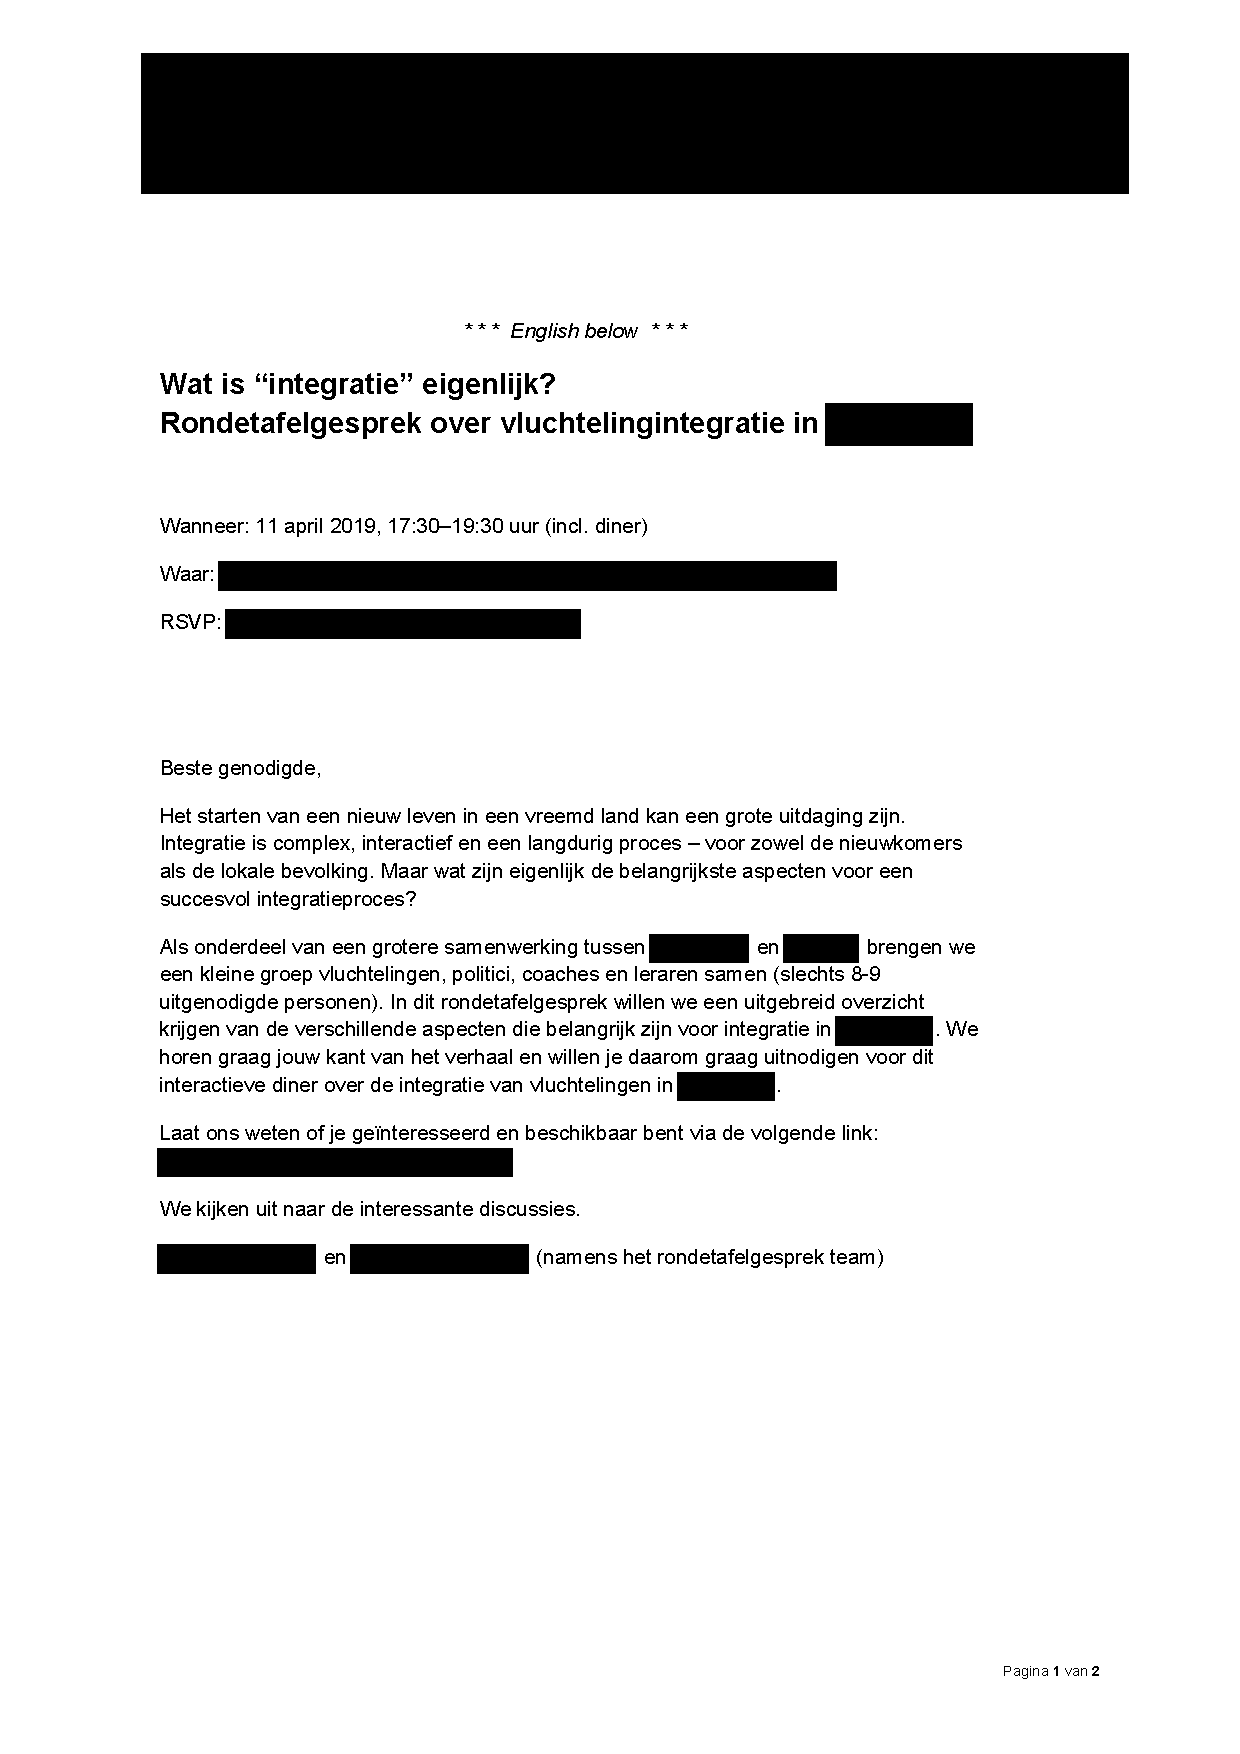
\includepdf[
    offset=0mm -15mm,
    clip=0mm 0mm 0mm 0mm,
    trim=0mm 0mm 0mm 0mm,
    pages=1,
    frame,
    scale=.80,
    pagecommand=\section{Materials: Round table invitation letter}\label{app:AppendixInvitation}
]{assets/Invitatie Ronde Tafel - Integratie in Groningen_redacted.pdf}

\includepdf[
    offset=0mm -10mm,
    clip=0mm 0mm 0mm 0mm,
    trim=0mm 0mm 0mm 0mm,
    pages=2,
    frame,
    scale=.80,
    pagecommand={}
]{assets/Invitatie Ronde Tafel - Integratie in Groningen_redacted.pdf}

\end{center}


\section{Materials: Semi-structured questions}\label{app:AppendixQuestions}

The following questions form the guiding structure of the focus group discussion. All three moderators received a copy of these questions to guide the discussion. We placed a particular focus on giving space to the natural discourse of the discussion and only referred back to these questions if a topic was saturated or the discussion digressed from the main topic too much. 

Next to the introductory section, the opening question, and the exit question, we organized the prepared questions around four topics: (a) the conceptual aspects of acculturation, (b) challenges to acculturation, (c) best practices of acculturation, and (d) the measurement of acculturation. While differing in abstraction and approach, all questions were aimed at exploring the conceptualization of psychological acculturation.

{\parindent0pt % disables indentation for all the text between { and }

\textbf{Welcome:}
\begin{itemize}[noitemsep,topsep=0pt]
    \item General introduction of the project
    \item Aim of evening
    \item Informed consent
\end{itemize}

\textbf{Introduction participants:}
\begin{itemize}[noitemsep,topsep=0pt]
    \item Name
    \item Background
\end{itemize}

\textbf{Opening Question:}
\begin{enumerate}[noitemsep,topsep=0pt]
    \item [(1.)] How do you see integration in your daily life?
\end{enumerate}

\textbf{Aspects / Elements:}
\begin{enumerate}[noitemsep,topsep=0pt]
    \item [(2.)] What does integration mean to you?\newline
    \textit{Clarification:} Based on your experience, what are the most important aspects of integration?\newline
    \textit{Alternative formulation:} What does successful integration look like to you?
    \item [(3.)] Who should be involved in integration?\newline
    \textit{Follow-up question:} What roles do these groups have?
    \item [(4.)] What do you expect from refugees and what from Dutch people?\newline
    \textit{Clarification:} What can Dutch society do?\newline
    \textit{Alternative formulations:} How are the Dutch influenced by integration? How can the Dutch contribute to integration? What is the role of the Dutch in integration?
\end{enumerate}

\textbf{Challenges:}
\begin{enumerate}[noitemsep,topsep=0pt]
    \item [(5.)] What are the biggest challenges for refugees coming to the Netherlands?\newline
    \textit{Alternative formulation:} What doesn't work so well?\newline
    \textit{Follow-up question:} What is the biggest challenge to (becoming a part of Dutch culture / or another key element identified earlier)?
    \item [(6.)] What are the biggest challenges for Dutch people who receive refugees?
\end{enumerate}

\textbf{Support:}
\begin{enumerate}[noitemsep,topsep=0pt]
    \item [(7.)] What works well?
    \item [(8.)] How can we facilitate integration?\newline
    \textit{Alternative formulation:} How can we improve integration?
\end{enumerate}

\textbf{Measurement question:}
\begin{enumerate}[noitemsep,topsep=0pt]
    \item [(9.)] What should we absolutely ask/include in the survey?\newline
    \textit{Alternative formulations:} What aspects of integration should we pay attention to if we want to measure integration? What should we not miss? From your experience what is the most important question (to add to a survey)?
    \item [(10.)] Which challenges do you see for measuring integration?
\end{enumerate}

\textbf{Exit question:} 
\begin{enumerate}[noitemsep,topsep=0pt]
    \item [(11.)] Is there anything else you would like to say?
\end{enumerate}

}

\end{document}